\documentclass[11pt,letterpaper]{article}

% PAQUETES
\usepackage[utf8]{inputenc}
\usepackage[T1]{fontenc}
\usepackage[spanish,es-tabla]{babel}
\usepackage[margin=2.3cm]{geometry}
\usepackage{amsmath,amssymb}
\usepackage{booktabs}
\usepackage{graphicx}
\usepackage{float}
\usepackage{tabularx}
\usepackage[hidelinks]{hyperref}
\usepackage[expansion=false]{microtype}

% FORMATO
\setlength{\parindent}{0pt}
\setlength{\parskip}{7pt}
\setlength{\emergencystretch}{3em}
\renewcommand{\arraystretch}{1.15}
\graphicspath{{figuras/}}

% IMÁGENES QUE DEBES SUBIR A LA CARPETA figuras:
% simulaciones.png
% tendencia.png
% estacionalidad.png
% acf_ventas.png
% acf_ols.png
% acf_ar1.png
% pronosticos.png

\newcommand{\figura}[3][0.94]{
    \begin{figure}[H]
        \centering
        \includegraphics[width=#1\linewidth]{#2}
        \caption{#3}
    \end{figure}
}

\begin{document}

% PORTADA
\begin{titlepage}
    \centering
    \vspace*{2cm}

    {\Large Universidad del Istmo de Guatemala\par}
    \vspace{0.5cm}

    {\large Facultad de Ingeniería\par}
    \vspace{2cm}

    {\LARGE\bfseries Business Intelligence\par}
    \vspace{0.7cm}

    {\Large Tarea 4\par}
    \vspace{0.4cm}

    {\Large Introducción a series de tiempo\par}

    \vfill

    {\large Maria Olga Menegazzo Obiols\par}
    \vspace{1cm}

    {\large 25 de octubre de 2026\par}

    \vspace*{1cm}
\end{titlepage}

\section*{Introducción}

Para esta tarea trabajé con las ventas de Online Retail. Primero hice las simulaciones para entender qué pasa cuando una serie tiene memoria y qué pasa cuando cambia su media. Después limpié los datos, revisé el calendario y analicé la tendencia y la estacionalidad de las ventas.

También comparé diferentes modelos de pronóstico, tomando en cuenta que para predecir una venta solo se puede usar la información disponible hasta ese momento. Finalmente, hice el análisis RFM para conocer mejor a los clientes y ver qué características se relacionan con una mayor probabilidad de volver a comprar.

\section*{Parte 0. Procesos simulados}

\subsection*{0.1. Derivación del AR(1)}

Parto del proceso:
\[
Y_t=c+\phi Y_{t-1}+\varepsilon_t,
\]
donde las innovaciones son independientes del pasado, tienen media cero y varianza $\sigma^2$.

Si $|\phi|<1$ y el proceso es estacionario, su media es constante. Entonces:
\[
\mathbb{E}(Y_t)
=
c+\phi\mathbb{E}(Y_{t-1})
+\mathbb{E}(\varepsilon_t).
\]

Como la media de las innovaciones es cero:
\[
\mu=c+\phi\mu.
\]

Al despejar:
\[
\mu(1-\phi)=c,
\]
por lo que:
\[
\boxed{\mathbb{E}(Y_t)=\frac{c}{1-\phi}}.
\]

Para obtener la varianza, uso que la innovación es independiente del pasado:
\[
\operatorname{Var}(Y_t)
=
\phi^2\operatorname{Var}(Y_{t-1})+\sigma^2.
\]

Por estacionariedad, la varianza de ambos períodos es la misma:
\[
v=\phi^2v+\sigma^2.
\]

Entonces:
\[
v(1-\phi^2)=\sigma^2,
\]
y obtengo:
\[
\boxed{\operatorname{Var}(Y_t)=\frac{\sigma^2}{1-\phi^2}}.
\]

Para la autocorrelación, primero centro el proceso:
\[
Y_t-\mu=\phi(Y_{t-1}-\mu)+\varepsilon_t.
\]

Para $k\geq1$, la innovación no tiene covarianza con $Y_{t-k}$. Por eso:
\[
\gamma_k
=
\operatorname{Cov}(Y_t,Y_{t-k})
=
\phi\gamma_{k-1}.
\]

Al repetir esta relación:
\[
\gamma_k=\phi^k\gamma_0.
\]

Como:
\[
\rho_k=\frac{\gamma_k}{\gamma_0},
\]
queda:
\[
\boxed{\rho_k=\phi^k}.
\]

En la caminata aleatoria, con $\phi=1$, $c=0$ y $Y_0=0$:
\[
Y_t=Y_{t-1}+\varepsilon_t
=
\sum_{j=1}^{t}\varepsilon_j.
\]

Como las innovaciones son independientes:
\[
\operatorname{Var}(Y_t)
=
\sum_{j=1}^{t}\operatorname{Var}(\varepsilon_j)
=
\boxed{t\sigma^2}.
\]

La varianza aumenta con el tiempo, por lo que la caminata aleatoria no es débilmente estacionaria. A diferencia del AR(1) estacionario, no tiene una varianza constante alrededor de la cual se mantenga la serie.

\subsection*{0.2. Simulación}

Simulé 300 observaciones de cada proceso y descarté los primeros 200 pasos. Utilicé 5\,000 réplicas para cada valor de $\phi$, con las semillas 100, 101, 102 y 103 para $\phi=0$, $0.5$, $0.9$ y $1$, respectivamente.

Para las realizaciones ilustrativas utilicé la semilla 1 en cada escenario.

El error estándar de Monte Carlo de cada promedio se calculó como:
\[
EE(\bar{x})=\frac{s_x}{\sqrt{5000}}.
\]

\begin{table}[H]
\centering
\small
\caption{Resultados de las simulaciones AR(1). El error estándar aparece entre paréntesis.}
\resizebox{\linewidth}{!}{
\begin{tabular}{rrrrrr}
\toprule
$\phi$
& Promedio $r_1$
& Promedio $r_5$
& $\phi^5$
& Rechazo, rezago 1
& Promedio $\widehat{\phi}$\\
\midrule

0
& $-0.003491\ (0.000827)$
& $-0.002905\ (0.000804)$
& 0
& $0.0498\ (0.003077)$
& $-0.003495\ (0.000829)$\\

0.5
& $0.490839\ (0.000710)$
& $0.018137\ (0.001017)$
& 0.03125
& $1.0000\ (0.000000)$
& $0.492551\ (0.000712)$\\

0.9
& $0.883286\ (0.000400)$
& $0.532695\ (0.001423)$
& 0.59049
& $1.0000\ (0.000000)$
& $0.886509\ (0.000396)$\\

1
& $0.975487\ (0.000209)$
& $0.881910\ (0.000942)$
& $1^{*}$
& $1.0000\ (0.000000)$
& $0.981973\ (0.000215)$\\

\bottomrule
\end{tabular}
}
\end{table}

El asterisco indica que, para la caminata aleatoria, $\phi^5=1$ es únicamente una referencia algebraica. La fórmula de autocorrelación del proceso estacionario no se puede extender directamente a este caso.

Los errores estándar de rechazo iguales a cero aparecen porque todas las réplicas rechazaron. Esto no significa que la probabilidad poblacional se conozca sin incertidumbre.


\begin{figure}
    \centering
    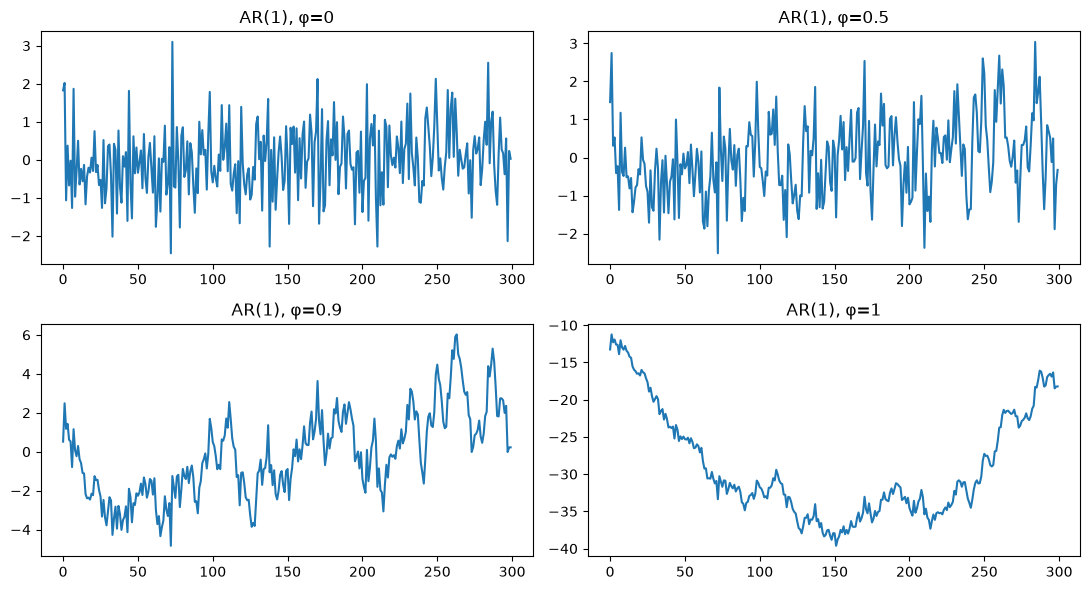
\includegraphics[width=0.5\linewidth]{simulaciones.png}
    \caption{Enter Caption}
    \label{fig:placeholder}
\end{figure}
Realizaciones de los cuatro procesos. Cuando $\phi$ se acerca a uno, los movimientos duran más y la serie presenta mayor persistencia.
}

\subsection*{0.3. Interpretación}

Para ruido blanco, la tasa de rechazo fue de 4.98\%, muy cercana al 5\% esperado con las bandas:
\[
\pm\frac{1.96}{\sqrt{300}}.
\]

Esto tiene sentido porque, cuando $\phi=0$, una observación no depende de la anterior.

En las simulaciones, OLS tiende a estimar un valor un poco menor al verdadero. La diferencia aumenta cuando $\phi$ se acerca a uno. Para $\phi=0.9$, el promedio estimado fue 0.886509, mientras que para la caminata aleatoria fue 0.981973.

Este sesgo en una muestra de tamaño fijo no demuestra que el estimador sea inconsistente. La consistencia se refiere a lo que ocurre cuando aumenta el tamaño de la muestra, no cuando se repite más veces una muestra de 300 observaciones.

Para la caminata aleatoria, el promedio de $r_5$ fue 0.881910, menor que uno. Aquí influyen la no estacionariedad, el uso de la media muestral y la normalización de la autocorrelación.

Descartar 200 observaciones no vuelve estacionaria a la caminata aleatoria. Sin embargo, el nivel acumulado antes de la ventana funciona como un desplazamiento común. Al restar la media para calcular $r_k$, ese desplazamiento desaparece.

\subsection*{0.4. Procesos con una media que cambia}

También simulé procesos con innovaciones independientes y una media determinista:
\[
Y_t=m_t+\varepsilon_t.
\]

Para la tendencia utilicé:
\[
m_t=\frac{2t}{300}.
\]

Para el patrón semanal:
\[
m_t=
\begin{cases}
-1.5, & t\bmod7=6,\\
0.25, & \text{en los demás días}.
\end{cases}
\]

Utilicé las semillas 200 para tendencia, 201 para el patrón semanal y 300 para el ruido blanco de comparación.

\begin{table}[H]
\centering
\small
\caption{Resultados de los procesos con innovaciones independientes. Los errores estándar aparecen entre paréntesis.}
\resizebox{\linewidth}{!}{
\begin{tabular}{lrrrr}
\toprule
Escenario
& Promedio $r_1$
& Rechazo, rezago 1
& Promedio $r_7$
& Rechazo LB(10)\\
\midrule

Tendencia
& 0.245198
& $0.9822\ (0.001870)$
& $0.230659\ (0.000819)$
& $1.0000\ (0.000000)$\\

Semanal
& $-0.048201$
& $0.1170\ (0.004546)$
& $0.265660\ (0.000833)$
& $0.9522\ (0.003017)$\\

Ruido blanco
& $-0.003196$
& $0.0502\ (0.003088)$
& $-0.003122\ (0.000803)$
& $0.0512\ (0.003117)$\\

\bottomrule
\end{tabular}
}
\end{table}

La tendencia provoca rechazo en casi todas las réplicas, aunque las innovaciones no tengan memoria. Esto ocurre porque la media cambia y las observaciones cercanas suelen quedar del mismo lado de la media general.

El patrón semanal pasa la prueba de rezago 1 en la mayoría de las réplicas, aunque rechaza en 11.7\%. Su estructura aparece con mayor claridad en el rezago 7.

Esto se relaciona con lo que vimos con RANDU. Que una prueba no detecte un problema no significa que los datos no tengan estructura. Puede ser que se esté revisando una relación que no permite verla.

\subsection*{0.5. Prueba de Ljung--Box}

La prueba de Ljung--Box combina varios rezagos:
\[
Q(m)
=
n(n+2)
\sum_{k=1}^{m}
\frac{r_k^2}{n-k}.
\]

Con diez rezagos, detectó el patrón semanal en 95.22\% de las réplicas. Esto es mucho más que el 11.7\% de la prueba de rezago 1.

Para la tendencia rechazó en todas las réplicas y, para ruido blanco, mantuvo una tasa cercana al 5\%.

La implementación manual coincidió con la de \texttt{statsmodels}. Para la muestra de comparación, ambas dieron:
\[
Q(10)=18.139395,
\qquad
p=0.052657.
\]

La diferencia principal es que Ljung--Box permite identificar estructura en varios rezagos al mismo tiempo, mientras que revisar solamente el primero puede dejar pasar un patrón semanal.

\section*{Parte 1. Limpieza}

\subsection*{1.1. Revisión inicial}

El archivo original contiene:
\begin{itemize}
    \item 541\,909 filas.
    \item 25\,900 facturas.
    \item 4\,070 códigos de producto.
    \item 4\,372 clientes identificados.
\end{itemize}

Cargué \texttt{InvoiceNo}, \texttt{StockCode} y \texttt{CustomerID} como texto porque son identificadores. Pueden contener prefijos y no representan cantidades con las que tenga sentido realizar operaciones aritméticas.

Las filas sin cliente corresponden a 3\,710 facturas y suman aproximadamente \pounds1\,447\,682 antes de aplicar la limpieza.

\subsection*{1.2. Decisiones de limpieza}

\textbf{Duplicados exactos.}

Eliminé 5\,268 filas duplicadas exactas para evitar contar dos veces una misma línea.

\textbf{Prefijos de las facturas.}

Conservé las facturas que empiezan con C porque representan cancelaciones y deben restar el día en que ocurren. Eliminé las facturas con prefijo A, identificadas como ajustes de deuda.

\textbf{Códigos que no representan productos.}

Utilicé como regla conservar los códigos que comienzan con cinco dígitos o con \texttt{DCGS}. Esta decisión toma en cuenta que algunos códigos con un formato distinto también pueden representar productos.

Conservé además los créditos manuales \texttt{M} en facturas C. Esta excepción evita mantener una venta sin reconocer que después fue devuelta mediante un crédito manual.

\textbf{Precios iguales a cero o negativos.}

Eliminé estas filas porque no representan una venta monetaria válida bajo la definición utilizada. En los datos originales hay 2\,515 filas con precio cero y dos con precio negativo.

\textbf{Cantidades negativas sin factura de cancelación.}

Encontré 1\,336 filas de este tipo. Todas tienen precio cero y varias descripciones se refieren a daños, revisiones o ajustes. En la bitácora final ya habían sido eliminadas por reglas anteriores.

\textbf{Filas sin cliente.}

Las conservé para el pronóstico agregado. Aunque no se sepa quién compró, la venta sí cuenta para el total. Solo las excluí del análisis RFM porque ahí necesito identificar a cada cliente.

\subsection*{1.3. Bitácora de limpieza}

\begin{table}[H]
\centering
\small
\caption{Bitácora secuencial de limpieza. Los montos corresponden a las filas retiradas, con su signo original y en libras.}
\begin{tabularx}{\linewidth}{Xrr}
\toprule
Regla & Filas retiradas & Monto retirado\\
\midrule

Duplicados exactos
& 5\,268
& 21\,740.980\\

Prefijo distinto de dígito o C
& 3
& $-11\,062.060$\\

Códigos no producto, salvo créditos M/C
& 2\,697
& 112\,535.314\\

Precio menor o igual a cero
& 2\,492
& 0.000\\

Cantidad negativa sin cancelación
& 0
& 0.000\\

\midrule

Total retirado
& 10\,460
& 123\,214.234\\

Filas finales
& 531\,449
& ---\\

\bottomrule
\end{tabularx}
\end{table}

Los conteos dependen del orden de las reglas. Por ejemplo, las 2\,492 filas con precio no positivo de esta tabla son las que todavía estaban presentes después de aplicar los filtros anteriores.

\subsection*{Pedidos extremos y créditos manuales}

Las facturas 541431 y C541433 registran una venta y una cancelación de \pounds77\,183.60 el mismo día. Las facturas 581483 y C581484 hacen lo mismo por \pounds168\,469.60. Conservé ambas parejas porque se compensan al sumar la venta neta diaria.

El 10 de junio de 2011 aparece una venta por \pounds38\,970 en la factura 556444 y un crédito manual del mismo importe en C556445. Si se eliminan todos los códigos M, la devolución desaparece y la venta queda sobrestimada.

La limpieza final conserva 244 créditos M/C, con un monto conjunto aproximado de $-\text{\pounds}146\,784$.

No eliminé todas las ventas grandes solo por su tamaño. Primero revisé si tenían una cancelación o un ajuste relacionado.

\section*{Parte 2. El calendario}

\subsection*{2.1. Construcción de la serie diaria}

La venta neta diaria se calculó como:
\[
y_d=
\sum_{i:\,\operatorname{fecha}(i)=d}
\texttt{Quantity}_i\texttt{UnitPrice}_i.
\]

Entre el 1 de diciembre de 2010 y el 9 de diciembre de 2011 hay 374 días calendario. En 305 hubo al menos una transacción.

Faltan 69 fechas: 53 sábados y 16 días adicionales.

\subsection*{2.2. Días sin transacciones}

\begin{table}[H]
\centering
\small
\caption{Días sin transacciones, aparte de los sábados.}
\begin{tabularx}{\linewidth}{p{0.39\linewidth}X}
\toprule
Fechas & Clasificación\\
\midrule

24, 26, 27, 28, 29, 30 y 31 de diciembre de 2010
&
Intervalo sin operaciones alrededor de Navidad, con feriados sustitutos y cierres adicionales de la tienda.
\\

2 y 3 de enero de 2011
&
Intervalo de Año Nuevo, incluido el feriado sustituto del lunes.
\\

22, 24 y 25 de abril de 2011
&
Viernes Santo, domingo de Pascua y lunes de Pascua.
\\

29 de abril de 2011
&
Feriado extraordinario por la boda real.
\\

2 y 30 de mayo de 2011
&
Feriados bancarios de mayo.
\\

29 de agosto de 2011
&
Feriado bancario de verano.
\\

\bottomrule
\end{tabularx}
\end{table}

La tienda no registra transacciones los sábados. Además, hay cierres relacionados con Navidad, Año Nuevo y los feriados bancarios.

El 29 de abril fue un caso especial porque se declaró feriado por la boda del príncipe William y Catherine Middleton \cite{boda}.

Los cierres de Semana Santa son móviles porque la fecha de Pascua cambia entre años. No todos los días del intervalo navideño son feriados oficiales, por lo que también hay días que corresponden a cierres adicionales de la tienda.

\subsection*{2.3. Cero o dato faltante}

La decisión depende del uso de la serie.

Si quiero medir ingresos por día calendario y sé que la tienda estuvo cerrada, ese día corresponde a cero.

Si quiero analizar cuánto vende la tienda cuando está abierta, lo represento como faltante y lo excluyo del ajuste. De esa manera, un cierre no se interpreta como un día normal en el que la demanda cayó a cero.

\subsection*{2.4. Último día del archivo}

El último registro es del 9 de diciembre de 2011 a las 12:50. Como el final del archivo puede dejar incompleto ese día, lo excluí del análisis.

Después de excluirlo quedaron:
\begin{itemize}
    \item 373 fechas calendario.
    \item 304 días abiertos.
    \item Ningún día abierto con venta neta menor o igual a cero.
    \item Una venta neta diaria mínima de \pounds3\,439.67.
\end{itemize}

El entrenamiento llega hasta el 30 de septiembre de 2011 y contiene 245 días abiertos.

La prueba evaluada empieza el 3 de octubre y termina el 8 de diciembre. El domingo 2 de octubre sirve como primer origen y como parte de la historia disponible, pero no se evalúa.

\section*{Parte 3. Tendencia, estacionalidad y autocorrelación}

\subsection*{3.1. Tendencia}

Calculé una media móvil centrada de siete días calendario. Para este cálculo rellené con cero los días sin operaciones.

Siete días cubren un ciclo semanal completo. Cinco no cubren toda la semana y treinta mezclan varios ciclos, por lo que suavizan más los cambios.

Al centrar la media móvil, esta queda alineada con el momento que describe. Sin embargo, utiliza observaciones futuras, así que sirve para describir la serie y no como predictor disponible en tiempo real.

\figura{tendencia.png}{
Venta neta diaria y media móvil centrada de siete días.
}

La serie presenta fluctuaciones importantes entre días y un nivel más alto hacia el final del período. Esto hace que los modelos entrenados principalmente con meses anteriores enfrenten una prueba distinta.

El comportamiento es compatible con una temporada de mayor demanda, pero un solo ciclo anual no permite confirmar una estacionalidad anual que se repita de la misma forma.

\subsection*{3.2. Índices estacionales}

Calculé el cociente entre la venta diaria y la media móvil:
\[
\frac{y_t}{MA_t}.
\]

Después promedié esos cocientes por día de la semana para las fechas de entrenamiento.

\begin{table}[H]
\centering
\caption{Índices estacionales por día de la semana.}
\begin{tabular}{lr}
\toprule
Día & Índice\\
\midrule
Lunes & 1.141\\
Martes & 1.547\\
Miércoles & 1.238\\
Jueves & 1.568\\
Viernes & 1.118\\
Domingo & 0.584\\
\bottomrule
\end{tabular}
\end{table}

\figura[0.8]{estacionalidad.png}{
Índices estacionales. Jueves y martes presentan los valores más altos, mientras que el domingo tiene el menor.
}

El promedio de los seis índices es 1.19946.

No tiene por qué ser exactamente uno porque la media móvil incluye siete días calendario y los cierres con cero, mientras que los índices se promedian únicamente entre los días abiertos. También influyen los cierres extraordinarios, la tendencia y el promedio de cocientes.

Los resultados muestran que jueves y martes tienen las ventas relativas más altas. El domingo presenta un nivel bastante menor.

Como la media móvil se calculó sobre el calendario completo, los cocientes cercanos al final de septiembre pueden incorporar días de octubre. Por eso estos índices tienen una interpretación descriptiva y no se utilizaron como predictores de los modelos de pronóstico.

\subsection*{3.3. Autocorrelación}

Implementé la autocorrelación con:
\[
r_k=
\frac{
\sum_{t=k+1}^{n}(y_t-\bar y)(y_{t-k}-\bar y)
}{
\sum_{t=1}^{n}(y_t-\bar y)^2
}.
\]

\figura{acf_ventas.png}{
ACF de los días abiertos del entrenamiento, con las bandas de referencia.
}

Con $n=245$, cinco de los 21 rezagos quedan fuera de las bandas. El rezago 1 también queda fuera, por lo que rechaza la prueba de ruido blanco.

El máximo aparece en el rezago 6. Cuando la semana tiene seis días abiertos, ese rezago representa una semana de siete días calendario. Esta equivalencia cambia cuando hay feriados o cierres adicionales.

Los resultados de Ljung--Box fueron:
\[
Q(6)=72.09595,
\qquad
p=1.52\times10^{-13},
\]
y:
\[
Q(12)=96.53305,
\qquad
p=2.65\times10^{-15}.
\]

Hay una estructura temporal clara. Sin embargo, no puedo atribuir toda esa autocorrelación a memoria. Como se vio en las simulaciones, los cambios de nivel y la estacionalidad también pueden producirla.

\section*{Parte 4. Del AR(1) al SARIMA}

\subsection*{4.1. Indicadores de día de la semana}

Ajusté las ventas por OLS usando seis indicadores de día de la semana, sin intercepto. Los residuos se calcularon como:
\[
e_t=y_t-X_t\widehat{\beta}.
\]

\figura{acf_ols.png}{
ACF de los residuos después de retirar los promedios por día de la semana.
}

Aunque quite el promedio de cada día de la semana, la serie todavía puede cambiar de nivel. Este modelo no incorpora una tendencia ni otros cambios en la media.

Por eso no basta con interpretar toda la autocorrelación restante como si siguiera la caída geométrica de un AR(1) estacionario. Los indicadores capturan diferencias entre días de la semana, pero no explican todos los movimientos de la serie.

\subsection*{4.2. AR(1) sobre los residuos}

Después ajusté:
\[
e_t=\widehat c+\widehat\phi e_{t-1}+u_t.
\]

El coeficiente estimado fue:
\[
\boxed{\widehat\phi=0.2773413}.
\]

\figura{acf_ar1.png}{
ACF de los residuos del AR(1). El ajuste reduce parte de la dependencia, pero no elimina toda la estructura.
}

Para los residuos $u_t$, usando un grado de libertad menos como indica la tarea, obtuve:
\[
Q(6)=26.30435,
\qquad
p=0.00007789,
\]
y:
\[
Q(12)=33.95432,
\qquad
p=0.00036796.
\]

Ambas pruebas rechazan ruido blanco al 5\%. Por lo tanto, el AR(1) no fue suficiente.

Esto muestra que explicar los promedios semanales y agregar una dependencia de un período todavía deja información en los residuos.

\subsection*{4.3. Ajuste SARIMA y convergencia}

Ajusté dos modelos sobre el logaritmo de las ventas:
\[
\mathrm{S1}:
\quad
\mathrm{SARIMA}(1,0,0)(1,0,0)_6
\quad
\text{con constante},
\]
y:
\[
\mathrm{S2}:
\quad
\mathrm{SARIMA}(0,1,1)(0,1,1)_6
\quad
\text{sin constante}.
\]

Usé un período de seis porque la serie contiene una observación por día abierto y normalmente hay seis días abiertos por semana.

Esta suposición se rompe cuando hay feriados. En esas semanas, seis observaciones consecutivas pueden abarcar más de siete días calendario.

El logaritmo ayuda a trabajar con cambios proporcionales y a reducir la influencia de variaciones grandes en el nivel de ventas. Pude aplicarlo porque todas las ventas diarias de la serie final son positivas.

\begin{table}[H]
\centering
\caption{Parámetros estimados con un máximo de 500 iteraciones.}
\begin{tabular}{lrr}
\toprule
Parámetro & S1 & S2\\
\midrule
Constante & 4.241856 & ---\\
AR(1) & 0.135526 & ---\\
AR estacional, rezago 6 & 0.514822 & ---\\
MA(1) & --- & $-0.910755$\\
MA estacional, rezago 6 & --- & $-0.683054$\\
Varianza de innovación & 0.218212 & 0.214490\\
\bottomrule
\end{tabular}
\end{table}

S1 no convergió con 50 iteraciones, pero sí con 500. Los parámetros cambiaron bastante:
\begin{itemize}
    \item La constante pasó de 1.464926 a 4.241856.
    \item El AR(1) pasó de 0.165562 a 0.135526.
    \item El AR estacional pasó de 0.822816 a 0.514822.
\end{itemize}

Por eso utilicé el ajuste con 500 iteraciones.

S2 convergió con ambos límites y mantuvo los mismos parámetros reportados. Los ajustes también convergieron en todos los orígenes móviles evaluados.

Para regresar los pronósticos a libras, apliqué la exponencial sin corrección de sesgo, como pide la tarea.

\subsection*{4.4. Diagnóstico de los residuos}

\begin{table}[H]
\centering
\caption{Ljung--Box sobre los residuos SARIMA, con $m-2$ grados de libertad.}
\begin{tabular}{lrrrr}
\toprule
Modelo & $Q(6)$ & Valor $p$ & $Q(12)$ & Valor $p$\\
\midrule
S1 & 9.352743 & 0.052863 & 23.042825 & 0.010590\\
S2 & 3.740357 & 0.442284 & 9.539814 & 0.481750\\
\bottomrule
\end{tabular}
\end{table}

En S2 descarté los primeros siete residuos por la inicialización de las diferencias.

S1 no rechaza ruido blanco al 5\% con seis rezagos, pero sí con doce. S2 no rechaza en ninguno de los dos casos.

Por estos resultados, S2 deja residuos más compatibles con ruido blanco. Esto favorece al modelo porque indica que logró capturar más de la estructura temporal de las ventas.

\subsection*{4.5. Pronósticos de largo plazo}

S1 es estacionario. Por eso sus pronósticos en logaritmos regresan a una media fija cuando aumenta el horizonte.

Con la transformación usada, el nivel límite en libras es aproximadamente:
\[
\exp\left(
\frac{4.241856}
{(1-0.135526)(1-0.514822)}
\right)
\approx
\text{\pounds}24\,658.
\]

Este valor corresponde a la exponencial de la media en logaritmos, sin corrección de sesgo.

S2 tiene diferencias ordinarias y estacionales. Por eso no está obligado a regresar a una media fija. Sus pronósticos dependen del nivel y del patrón estacional acumulados y pueden prolongar una trayectoria con cambio de nivel.

\section*{Parte 5. Pronóstico y fuga de información}

\subsection*{5.1. Modelos y evaluación}

Comparé los siguientes modelos:
\begin{itemize}
    \item \textbf{B1:} media histórica disponible.
    \item \textbf{B2:} última venta observada del mismo día de la semana.
    \item \textbf{M1:} tendencia lineal e indicadores de día de la semana.
    \item \textbf{M2:} indicadores y rezagos del mismo día de semanas anteriores.
    \item \textbf{S1 y S2:} los dos modelos SARIMA.
\end{itemize}

Para los rezagos semanales, cuando no había observación en la fecha buscada, retrocedí otra semana hasta encontrar una del mismo día. Por ejemplo, para el 9 de mayo, el rezago semanal retrocede hasta el 18 de abril.

En la evaluación temporal, cada domingo utilicé la historia disponible hasta ese día para pronosticar la semana siguiente.

La validación aleatoria utilizó cinco particiones y se repitió con diez semillas, de 0 a 9. Los orígenes internos van de mayo a septiembre. La prueba usa orígenes desde el 2 de octubre y termina el 8 de diciembre.

\subsection*{5.2. Comparación de errores}

\begin{table}[H]
\centering
\small
\caption{Errores en libras. En la validación aleatoria se reporta media $\pm$ desviación estándar entre semillas.}
\resizebox{\linewidth}{!}{
\begin{tabular}{lrrrrrr}
\toprule

&
\multicolumn{2}{c}{(a) Aleatoria}
&
\multicolumn{2}{c}{(b) Temporal interna}
&
\multicolumn{2}{c}{(c) Prueba temporal}\\

Modelo & MAE & RMSE & MAE & RMSE & MAE & RMSE\\
\midrule

B1
& $10\,274\pm51$
& $14\,191\pm47$
& 10\,177
& 14\,812
& 22\,233
& 26\,979\\

B2
& ---
& ---
& 11\,138
& 15\,414
& 14\,563
& 18\,765\\

M1
& $9\,147\pm116$
& $12\,524\pm103$
& 9\,757
& 13\,816
& 15\,395
& 20\,455\\

M2
& $8\,359\pm109$
& $11\,763\pm205$
& 9\,172
& 13\,263
& 15\,384
& 20\,076\\

S1
& ---
& ---
& 9\,615
& 13\,655
& 16\,757
& 21\,160\\

S2
& ---
& ---
& 9\,889
& 13\,840
& \textbf{12\,777}
& \textbf{16\,008}\\

\bottomrule
\end{tabular}
}
\end{table}

Al dividir los datos al azar, el modelo puede aprender de fechas posteriores a las que estoy evaluando. Esto no reproduce la situación real de pronosticar con información disponible hasta una fecha concreta.

Para B2 y los modelos SARIMA, la secuencia temporal es parte de la definición del modelo. Por eso no corresponde aplicarles directamente estas particiones aleatorias.

En M1 y M2, la validación temporal interna se acerca más al error de prueba que la aleatoria. En B1, el MAE aleatorio es ligeramente más cercano, aunque el RMSE temporal es más cercano.

Ninguna de las evaluaciones internas refleja bien todo el aumento del error de prueba. Esto indica que el problema no se explica únicamente por la forma de dividir los datos.

\subsection*{5.3. Modelo ganador}

S2 obtiene el menor MAE y el menor RMSE de prueba:
\[
\boxed{MAE=12\,777},
\qquad
\boxed{RMSE=16\,008}.
\]

Su MAE es aproximadamente 12.3\% menor que el de B2.

El diagnóstico de residuos también favorece a S2. Las diferencias y los términos MA permiten capturar estructura que todavía quedaba en S1.

El mejor modelo en la evaluación temporal interna era M2, pero en prueba ganó S2. Esto muestra que el resultado dentro del entrenamiento no siempre se mantiene cuando cambia el período evaluado.

\figura{pronosticos.png}{
Pronósticos semanales frente a las ventas observadas de octubre a diciembre.
}

La gráfica permite comparar qué tan bien sigue cada modelo los cambios en las ventas. En conjunto con los errores de prueba, S2 fue el que logró un mejor desempeño durante este período.

\subsection*{5.4. La trampa de la media móvil centrada}

Agregué a M2 la media móvil centrada de siete días. Los errores aparentes mejoraron:

\begin{table}[H]
\centering
\small
\caption{Comparación de M2 con y sin media móvil centrada.}
\resizebox{\linewidth}{!}{
\begin{tabular}{lrrrr}
\toprule

&
\multicolumn{2}{c}{Aleatoria}
&
\multicolumn{2}{c}{Temporal interna}\\

Modelo & MAE & RMSE & MAE & RMSE\\
\midrule

M2
& $8\,359\pm109$
& $11\,763\pm205$
& 9\,172
& 13\,263\\

M2 con MA centrada
& $7\,405\pm87$
& $10\,037\pm145$
& 8\,288
& 11\,176\\

\bottomrule
\end{tabular}
}
\end{table}

No se puede usar este predictor para un pronóstico real porque la ventana centrada contiene la propia venta objetivo y ventas futuras que todavía no se conocen al emitir el pronóstico.

El origen móvil no corrige este problema si la media móvil se calcula una sola vez sobre toda la serie y después se consulta en cada fecha.

Aunque el ajuste respete la fecha de corte, puede recibir información futura por medio de sus variables.

Por eso la mejora no representa una mayor capacidad real de pronóstico. Calcular la prueba de la misma forma produciría otra evaluación contaminada.

\subsection*{5.5. Causas del aumento del error}

La primera causa viene de cómo se dividen los datos. Si mezclo fechas, puedo permitir que el modelo aprenda del futuro. Esto se reduce usando orígenes temporales y construyendo los predictores con la información disponible en cada momento.

La segunda causa es que la serie cambia entre entrenamiento y prueba. En los meses finales aumenta el nivel de ventas y el modelo enfrenta un comportamiento distinto.

Aunque valide mejor, sigo sin tener otros años que me permitan ver cómo se comportan esos meses. Con aproximadamente un año tampoco hay suficientes ciclos para estimar y validar una estacionalidad anual de forma confiable.

\section*{Parte 6. Análisis RFM}

\subsection*{6.1. Construcción de R, F y M}

Utilicé las transacciones limpias con cliente identificado y anteriores al 1 de octubre de 2011.

Las variables se definieron así:
\begin{itemize}
    \item \textbf{Recencia:} días desde la última factura de venta, medidos al 1 de octubre.
    \item \textbf{Frecuencia:} número de facturas de venta distintas.
    \item \textbf{Monto:} venta neta acumulada, incluidas las cancelaciones.
\end{itemize}

Obtuve 3\,613 clientes con al menos una venta previa. Otros 44 clientes solo tienen cancelaciones antes del corte y no entran en la tabla RFM porque no tienen una última compra observada con la que pueda definir su recencia.

Doce clientes tienen $M\leq0$. Los conservé para mantener la información sobre devoluciones y no eliminar clientes únicamente por presentar un saldo neto no positivo.

No utilicé transacciones posteriores al corte para construir RFM porque eso introduciría información del mismo período cuya recompra quiero evaluar.

\subsection*{6.2. Puntajes por quintiles}

Para asignar los puntajes, primero ordené a los clientes por identificador. Después los barajé con la semilla 2026 y apliqué rangos con desempate por orden para dividir cada dimensión en cinco grupos.

En recencia invertí el signo para que cinco represente a los clientes que compraron más recientemente.

Cada puntaje tiene 722 o 723 clientes.

La frecuencia presenta muchos empates. Hay 1\,453 clientes que compraron una sola vez, por lo que los dos primeros quintiles de F contienen clientes con $F=1$ y el tercero también incluye algunos.

Dos clientes con la misma frecuencia pueden recibir puntajes distintos por el desempate aleatorio. Esto no significa que exista una diferencia real entre sus frecuencias de compra.

\subsection*{6.3. Recompra y AUC}

Definí recompra como haber realizado al menos una compra entre el 1 de octubre y el 8 de diciembre.

\begin{table}[H]
\centering
\caption{Fracción de clientes que volvió a comprar, por puntaje.}
\begin{tabular}{lrrrrr}
\toprule
Dimensión / puntaje & 1 & 2 & 3 & 4 & 5\\
\midrule
R & 0.278 & 0.381 & 0.553 & 0.665 & 0.663\\
F & 0.324 & 0.313 & 0.458 & 0.590 & 0.855\\
M & 0.295 & 0.374 & 0.454 & 0.608 & 0.809\\
\bottomrule
\end{tabular}
\end{table}

\begin{table}[H]
\centering
\caption{AUC para predecir recompra.}
\begin{tabular}{lr}
\toprule
Clasificador & AUC\\
\midrule
Recencia con signo invertido & 0.673\\
Frecuencia & 0.720\\
Monto & 0.709\\
Suma de los tres puntajes & 0.735\\
\bottomrule
\end{tabular}
\end{table}

Para los AUC individuales utilicé los valores crudos de R, F y M. En recencia invertí el signo porque un menor número de días representa una compra más reciente.

La tasa global de recompra fue de 50.8\%.

Frecuencia es la mejor dimensión individual por AUC. La suma de los puntajes mejora el resultado hasta 0.735, lo que indica que las tres dimensiones aportan información complementaria.

La separación no es perfectamente creciente en todos los casos. Por ejemplo, el puntaje cinco de recencia tiene una recompra ligeramente menor que el cuatro. En frecuencia, los primeros dos grupos contienen clientes empatados.

\subsection*{6.4. Clientes campeones}

Definí como campeones a los clientes con puntajes de cuatro o cinco en las tres dimensiones.

Representan:
\[
\boxed{21.6\%\text{ de los clientes RFM}}.
\]

Su participación en la venta neta posterior fue:
\[
\boxed{53.6\%}.
\]

Para calcular esta participación, el denominador incluye las ventas de todos los clientes identificados del período posterior, incluidos los nuevos.

Esto muestra que una parte relativamente pequeña de los clientes aporta más de la mitad de las ventas del período.

\subsection*{6.5. Clientes nuevos}

Los clientes sin ninguna factura de venta anterior al 1 de octubre generan 15.5\% de la venta neta posterior.

Son 723 clientes y aportan aproximadamente:
\[
\text{\pounds}368\,415
\]
de un total de:
\[
\text{\pounds}2\,376\,640.
\]

La definición incluye a quien no tenía ventas previas, aunque pudiera tener una cancelación anterior al corte.

Un modelo individual construido solo con clientes conocidos no puede asignar ventas a identidades que todavía no han aparecido. Para incluir ese componente necesitaría un modelo adicional de adquisición de clientes.

Un pronóstico agregado sí puede incorporar de forma implícita el flujo de clientes nuevos si su comportamiento histórico se mantiene, aunque no puede identificar quiénes serán.

Por eso, al comparar el enfoque agregado de la Parte 5 con uno cliente por cliente en el Proyecto 1, tengo que considerar las ventas que quedan fuera de la base RFM.

\section*{Conclusión}

Lo que más me quedó de esta tarea es que no basta con que un modelo tenga un error bajo. También hay que entender cómo se calculó ese error y si el modelo utilizó información que todavía no estaba disponible.

La limpieza también tuvo un efecto importante. Si hubiera eliminado todos los créditos manuales, algunas devoluciones habrían desaparecido y las ventas netas habrían quedado sobrestimadas.

En la prueba, S2 fue el modelo que mejor funcionó. Tuvo el menor MAE y RMSE, y sus residuos fueron más compatibles con ruido blanco en las pruebas realizadas.

Con RFM pude ver que los campeones aportan una parte importante de las ventas. Al mismo tiempo, los clientes nuevos tienen un peso que no puedo dejar fuera al construir un pronóstico. Por eso considero que el análisis agregado y el análisis por cliente se complementan y ayudan a entender distintas partes del negocio.

\begin{thebibliography}{9}

\bibitem{uci}
Chen, D.
\textit{Online Retail}.
UCI Machine Learning Repository, 2015.

\bibitem{rfm}
Chen, D., Sain, S. L. y Guo, K.
Data mining for the online retail industry: A case study of RFM model-based customer segmentation using data mining.
\textit{Journal of Database Marketing \& Customer Strategy Management},
19(3):197--208, 2012.

\bibitem{fpp}
Hyndman, R. J. y Athanasopoulos, G.
\textit{Forecasting: Principles and Practice}.
Segunda edición.
OTexts, 2018.

\bibitem{tsay}
Tsay, R. S.
\textit{Analysis of Financial Time Series}.
Segunda edición.
Wiley, 2005.

\bibitem{boda}
Prime Minister's Office, 10 Downing Street.
\textit{PM welcomes announcement of date for Royal wedding}.
23 de noviembre de 2010.
\url{https://www.gov.uk/government/news/pm-welcomes-announcement-of-date-for-royal-wedding}.

\end{thebibliography}

\end{document}
